\section{Theory}

\begin{figure}[t]
  \centering
  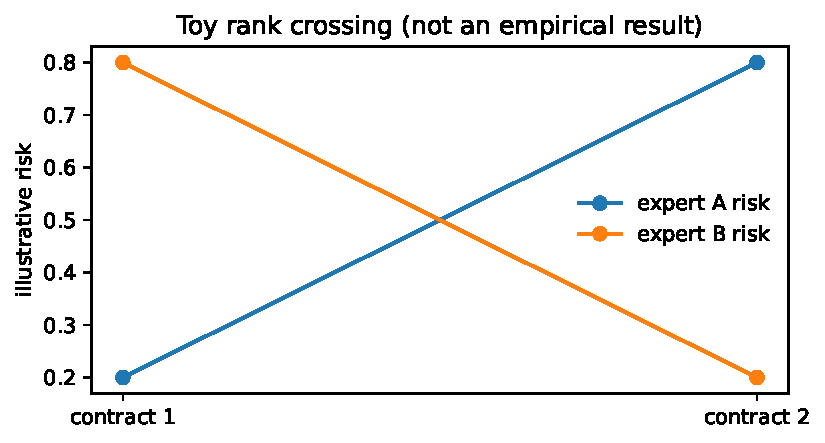
\includegraphics[width=.70\linewidth]{figures/figure_2_fixed_mixture_counterexample.pdf}
  \caption{Toy crossing-risk construction used to illustrate the
  fixed-mixture lower bound. Values are synthetic and not experiment results.}
  \label{fig:crossing}
\end{figure}

\begin{theorem}[Fixed-mixture regret; \texttt{PROVED}]
Consider two experts and two contracts. On contract one their risks are
$(0,\delta_1)$ and on contract two they are $(\delta_2,0)$, where
$\delta_1,\delta_2>0$. A contract-independent randomised mixture that selects
expert one with probability $w$ has worst-contract regret at least
\[
  \frac{\delta_1\delta_2}{\delta_1+\delta_2}>0.
\]
The bound is tight, while a contract-aware selector has zero regret.
\end{theorem}

\begin{proof}
The mixture regrets are $(1-w)\delta_1$ and $w\delta_2$. Their maximum is
minimised when they are equal, since decreasing either side of the intersection
increases the other maximum. Solving
$(1-w)\delta_1=w\delta_2$ gives
$w^\star=\delta_1/(\delta_1+\delta_2)$ and the stated value. A
contract-aware selector chooses expert one on contract one and expert two on
contract two.
\end{proof}

\paragraph{Failure of the premise.}
If either gap is zero, or one expert is optimal on both contracts, the positive
lower bound need not hold.

\begin{theorem}[Axis-additive approximation; \texttt{PROVED}]
Let the risk of a candidate routing action $a$ under a $d$-axis contract
$c=(c_1,\ldots,c_d)$ decompose as
\[
 R(a,c)=b(a)+\sum_{j=1}^d f_j(a,c_j)+h(a,c),
\]
where $|h(a,c)|\leq\epsilon_{\mathrm{int}}$. Suppose estimates satisfy
$|\widehat f_j(a,c_j)-f_j(a,c_j)|\leq\epsilon_j$ for every axis value present
in source contracts, and the learned router's optimisation error relative to
the minimiser of the estimated additive risk is at most
$\epsilon_{\mathrm{router}}$. For an unseen combination containing only those
observed axis values, its excess true risk over the best action is at most
\[
 2\sum_{j=1}^d\epsilon_j+
 2\epsilon_{\mathrm{int}}+\epsilon_{\mathrm{router}}.
\]
\end{theorem}

\begin{proof}
For any action, the difference between true risk and estimated additive risk is
at most $\sum_j\epsilon_j+\epsilon_{\mathrm{int}}$ by the triangle
inequality. Apply this bound once to the learned action and once to the true
optimal action, and insert the assumed optimisation error between their
estimated risks.
\end{proof}

\paragraph{Interpretation and counterexample.}
The guarantee does not cover an unseen axis value. It becomes vacuous when the
interaction residual is large. An XOR interaction between two contract axes
has zero marginal axis effects but nonzero joint risk, providing a direct
counterexample to factorisation without the residual term.


Both results are labelled \texttt{PROVED} in the proof audit. They concern
randomised expert selection risk and an axis-additive approximation class,
respectively; they do not establish real-world fraud performance. The appendix
states failure cases and numerical checks.
